\section{Architectural Design}
\subsection{Overview}
The system will be developed from scratch and the architectural choices that have been considered during the design of DREAM reflect the distributed nature of the system. Indeed, the functionalities offered by the system shall be used at the same time by various users located across the Telangana state. In order to maintain the scalability and ease to use experience of the application a three-tier approach has been implemented.\\
\begin{figure}[H]
    \centering
    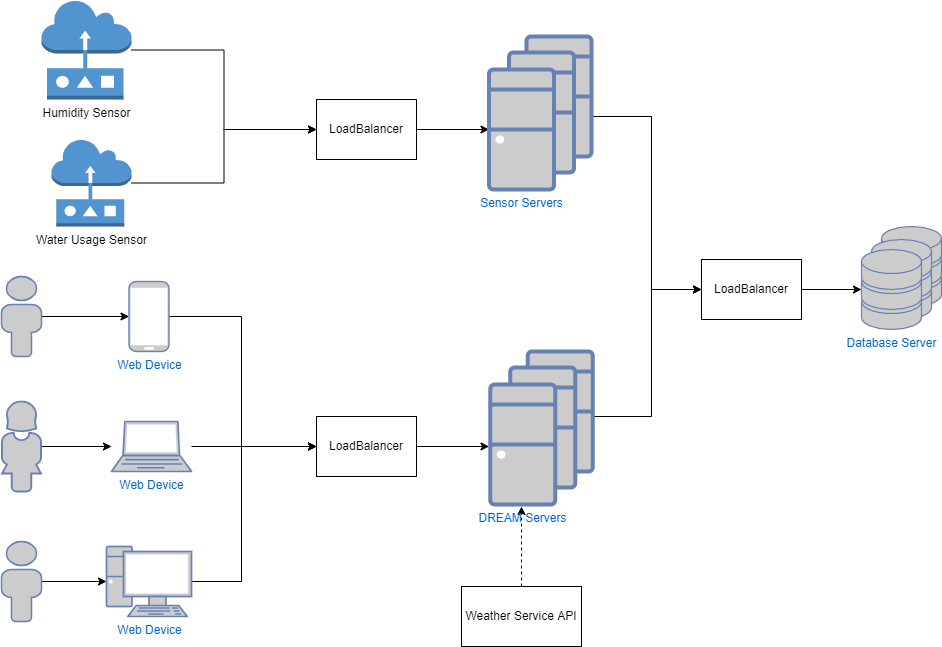
\includegraphics[scale=0.5]{Images/Components/OverviewDiagram.png}
    \caption{\textit{Overview Description}.}
\end{figure}
The high-level system consists of:
\begin{itemize}
    \item \textbf{Web Device:} Device enabled for internet connection and with a web browser installed to access the system. I.e., it can be a PC or a smartphone.
    \item \textbf{Water Usage Sensor:} Sensor used to detect the water consumed by a farmer.
    \item \textbf{Humidity Sensor:} Sensor used to detect moisture in the soil.
    \item \textbf{Weather Service API:} API used to access the weather information requested by the user.
    \item \textbf{Sensor Server:} Server used to manage communication between the sensors and the database.
    \item \textbf{DREAM Server:} Server where all the logic is located. It communicates with other servers and is the central point of the system.
    \item \textbf{Database Server:} Server where all the data are stored.
    \item \textbf{LoadBalancer:} Server with the only task of redirecting the load in an equal manner between the components.
\end{itemize}

\subsection{Component View}
\subsubsection{High Level}
The following component diagram highlights all the components of the system and describes both his internal and external interactions. A general overview of the whole system is shown in Figure.\\
\begin{figure}[H]
    \centering
    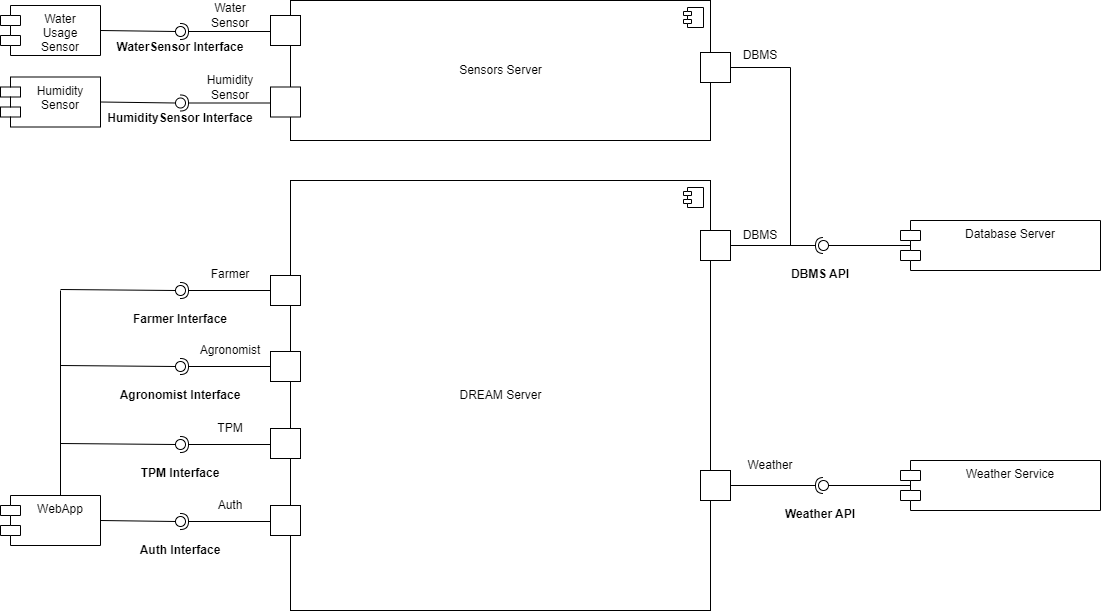
\includegraphics[scale=0.4]{Images/Components/ComponentDiagram - HL.png}
    \caption{\textit{High Level Overview}.}
\end{figure}
The components shown in Figure are:
\begin{itemize}
    \item \textbf{DREAM Server:}DREAM Server: it contains the business logic of the entire system. This component allows each user to use the services offered by DREAM, and also retrieves the data contained in the database and accesses the Telangana meteorological service.
    \item \textbf{WebApp} represents the interface with which users can access DREAM, via their preferred web browser. After the user has logged in via \textbf{Auth Interface}, it guarantees the correct access to the platform according to the functionalities that the user can use. I.e., \textbf{Farmer Interface} allows access to a farmer to "Report Production".
    \item \textbf{WaterUsageSensor} is a sensor that detects the flow of water flowing in a pipe. The sensor will be installed at the water supply point for each farmer in order to calculate his/ her exact consumption. The device is equipped with a 2G SIM to connect to DREAM and exchange information and to avoid excessive energy consumption.
    \item \textbf{HumiditySensor} is a sensor that detects the amount of moisture present in the soil. Each plot will be equipped with one of these sensors, and to make the user experience easier, sensors will be used that do not require a continuous source of electricity but can be self-sufficient through the use of mini solar panels. In addition, the device is equipped with a 2G SIM to connect to DREAM and exchange information, and to avoid excessive energy consumption.
    \item \textbf{Sensor Server} is the server responsible for communicating the data collected by the sensors distributed throughout Telangana and the database.
    \item \textbf{Database Server} provides the Sensor Server and DREAM Server with access to the data in the system.
    \item \textbf{Water Service} provides the interface to DREAM to retrieve the weather forecasts requested by a farmer or agronomist.
\end{itemize}
\subsubsection{DREAM Server}
The following component diagrams describe the internal structure of the application server, which contains the business logic of the system.\\
\begin{figure}[H]
    \centering
    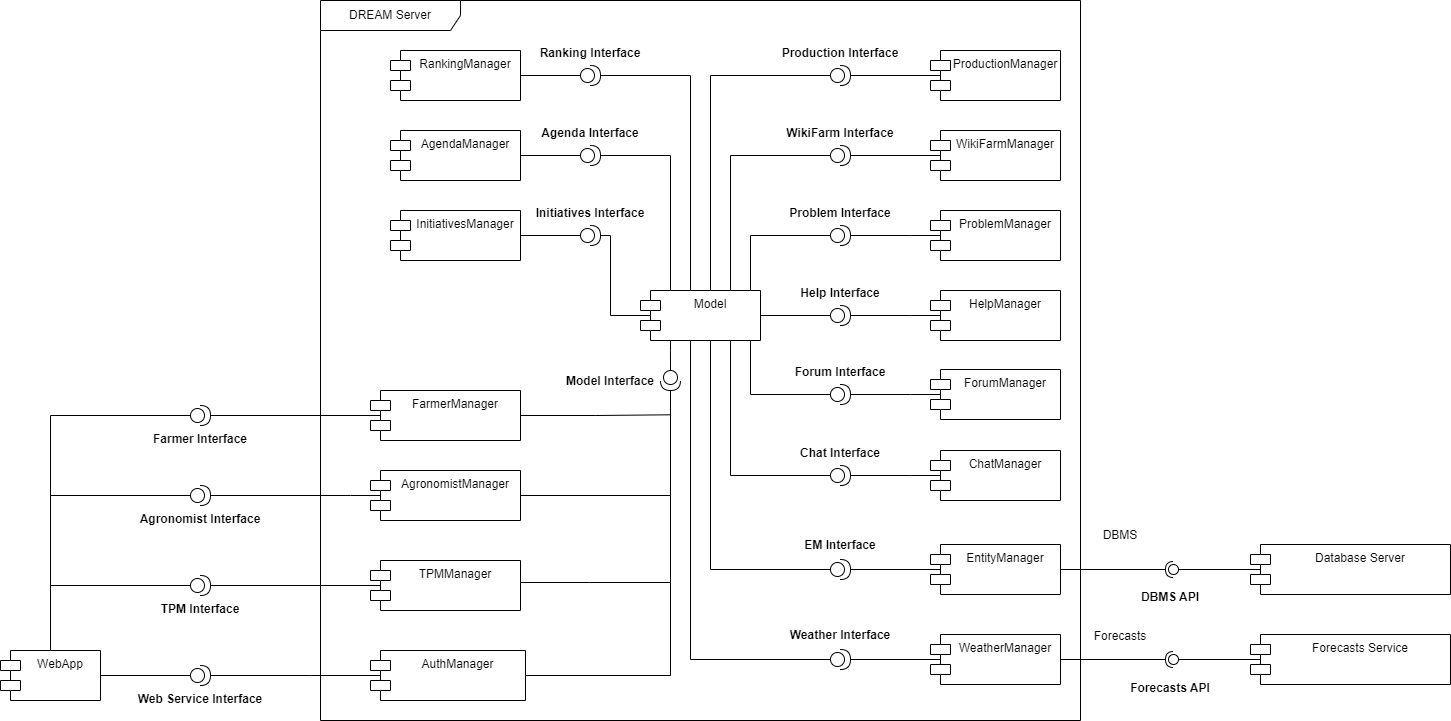
\includegraphics[scale=0.3]{Images/Components/ComponentDiagram - DREAMServer.png}
    \caption{\textit{DREAM Server Schema}.}
\end{figure}
The component used in the DREAM Server are:
\begin{itemize}
    \item \textbf{FarmerManager:} Component that manages the requests from a farmer's WebApp to functionality that it can access.
    \item \textbf{AgronomistManager:} Component that manages the requests from an agronomist WebApp to functionality that it can access.
    \item \textbf{TPMManager:} Component that manages the requests from a TPM WebApp to functionality that it can access.
    \item \textbf{AuthManager:} Component that verifies that the credentials entered by the user are correct.
    \item \textbf{Model:} This is the central component of DREAM Server. It generates the authentication token for each user and is responsible for managing all interactions between the server modules and, therefore, for querying the correct component according to the function desired by the user. In addition, it is the component that is responsible for querying the \textbf{EntityManager} and the \textbf{Telangana Weather Service API.}
    \item \textbf{RankingManager:} Component that computes with the ranking of the farmers present in an area selected by a user.
    \item \textbf{AgendaManager:} Component that allows manage the personal agenda of an agronomist. It allows to insert a new event, view the events scheduled for a selected day, confirm or modify an event saved in the diary and upload the report of a visit to a farmer that has just been completed.
    \item \textbf{InitiativesManager:} Component that allows a TPM to retrieve all the reports uploaded by agronomists to help a farmer.
    \item \textbf{Production Manager:} Component that allows a farmer to upload production data for his farm.
    \item \textbf{WikiFarm:} Component that suggests the most suitable fertilizers and seeds in the selected area.
    \item \textbf{ProblemManager:} Component that allows a farmer to upload details about a problem he/she has encountered. It also allows TPM and agronomists to view all the problems encountered by farmers in an area.
    \item \textbf{HelpManager:} Component that allows a farmer to enter a help request and allows agronomists and TPMs to view problems that have occurred in an area they have requested.
    \item \textbf{ForumManager:} Component that allows a farmer to create a new discussion or that allows him/her to reply to an already started discussion.
    \item \textbf{ChatManager:} Component that allows two users to communicate with each other.
    \item \textbf{EntityManager:} Component that allows two users to communicate with each other.
    \item \textbf{WeatherManager:} Component responsible for finding the weather forecast for a specific time slot requested by a user, by connecting to the Telangana weather portal.
\end{itemize}

\subsubsection{Sensor Server}
The following component diagrams describe the internal structure of the Sensor Server.\\
\begin{figure}[H]
    \centering
    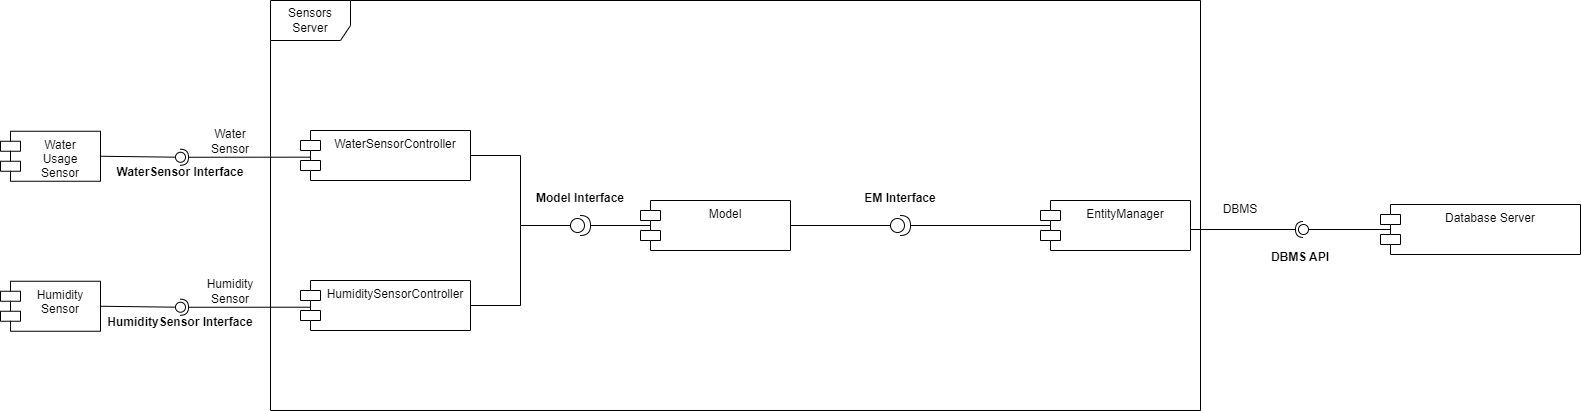
\includegraphics[scale=0.3]{Images/Components/ComponentDiagram - SensorServer.png}
    \caption{\textit{Sensor Server Schema}.}
\end{figure}
The component used in the Sensor Server are:
\begin{itemize}
    \item \textbf{WaterSensorController:} Component responsible for communication between the server and the water usage sensor
    \item \textbf{HumiditySensor: }Component responsible for communication between the server and the humidity sensor in a terrain.
    \item \textbf{Model: }It is the central component of the Sensor Server, it is responsible for managing the flow of information between the sensors to the EntityManager.
    \item \textbf{EntityManager: }Component responsible for managing the interactions between the database and the Sensor Server.
\end{itemize}
\newpage
\subsection{Deployment view}
In the following section, the deployment of DREAM is discussed with the visual help of a deployment diagram. This architecture offers three tiers, which are separated by two layers of load balancers. This choice will be motivated in the following section.\\
\begin{figure}[H]
    \centering
    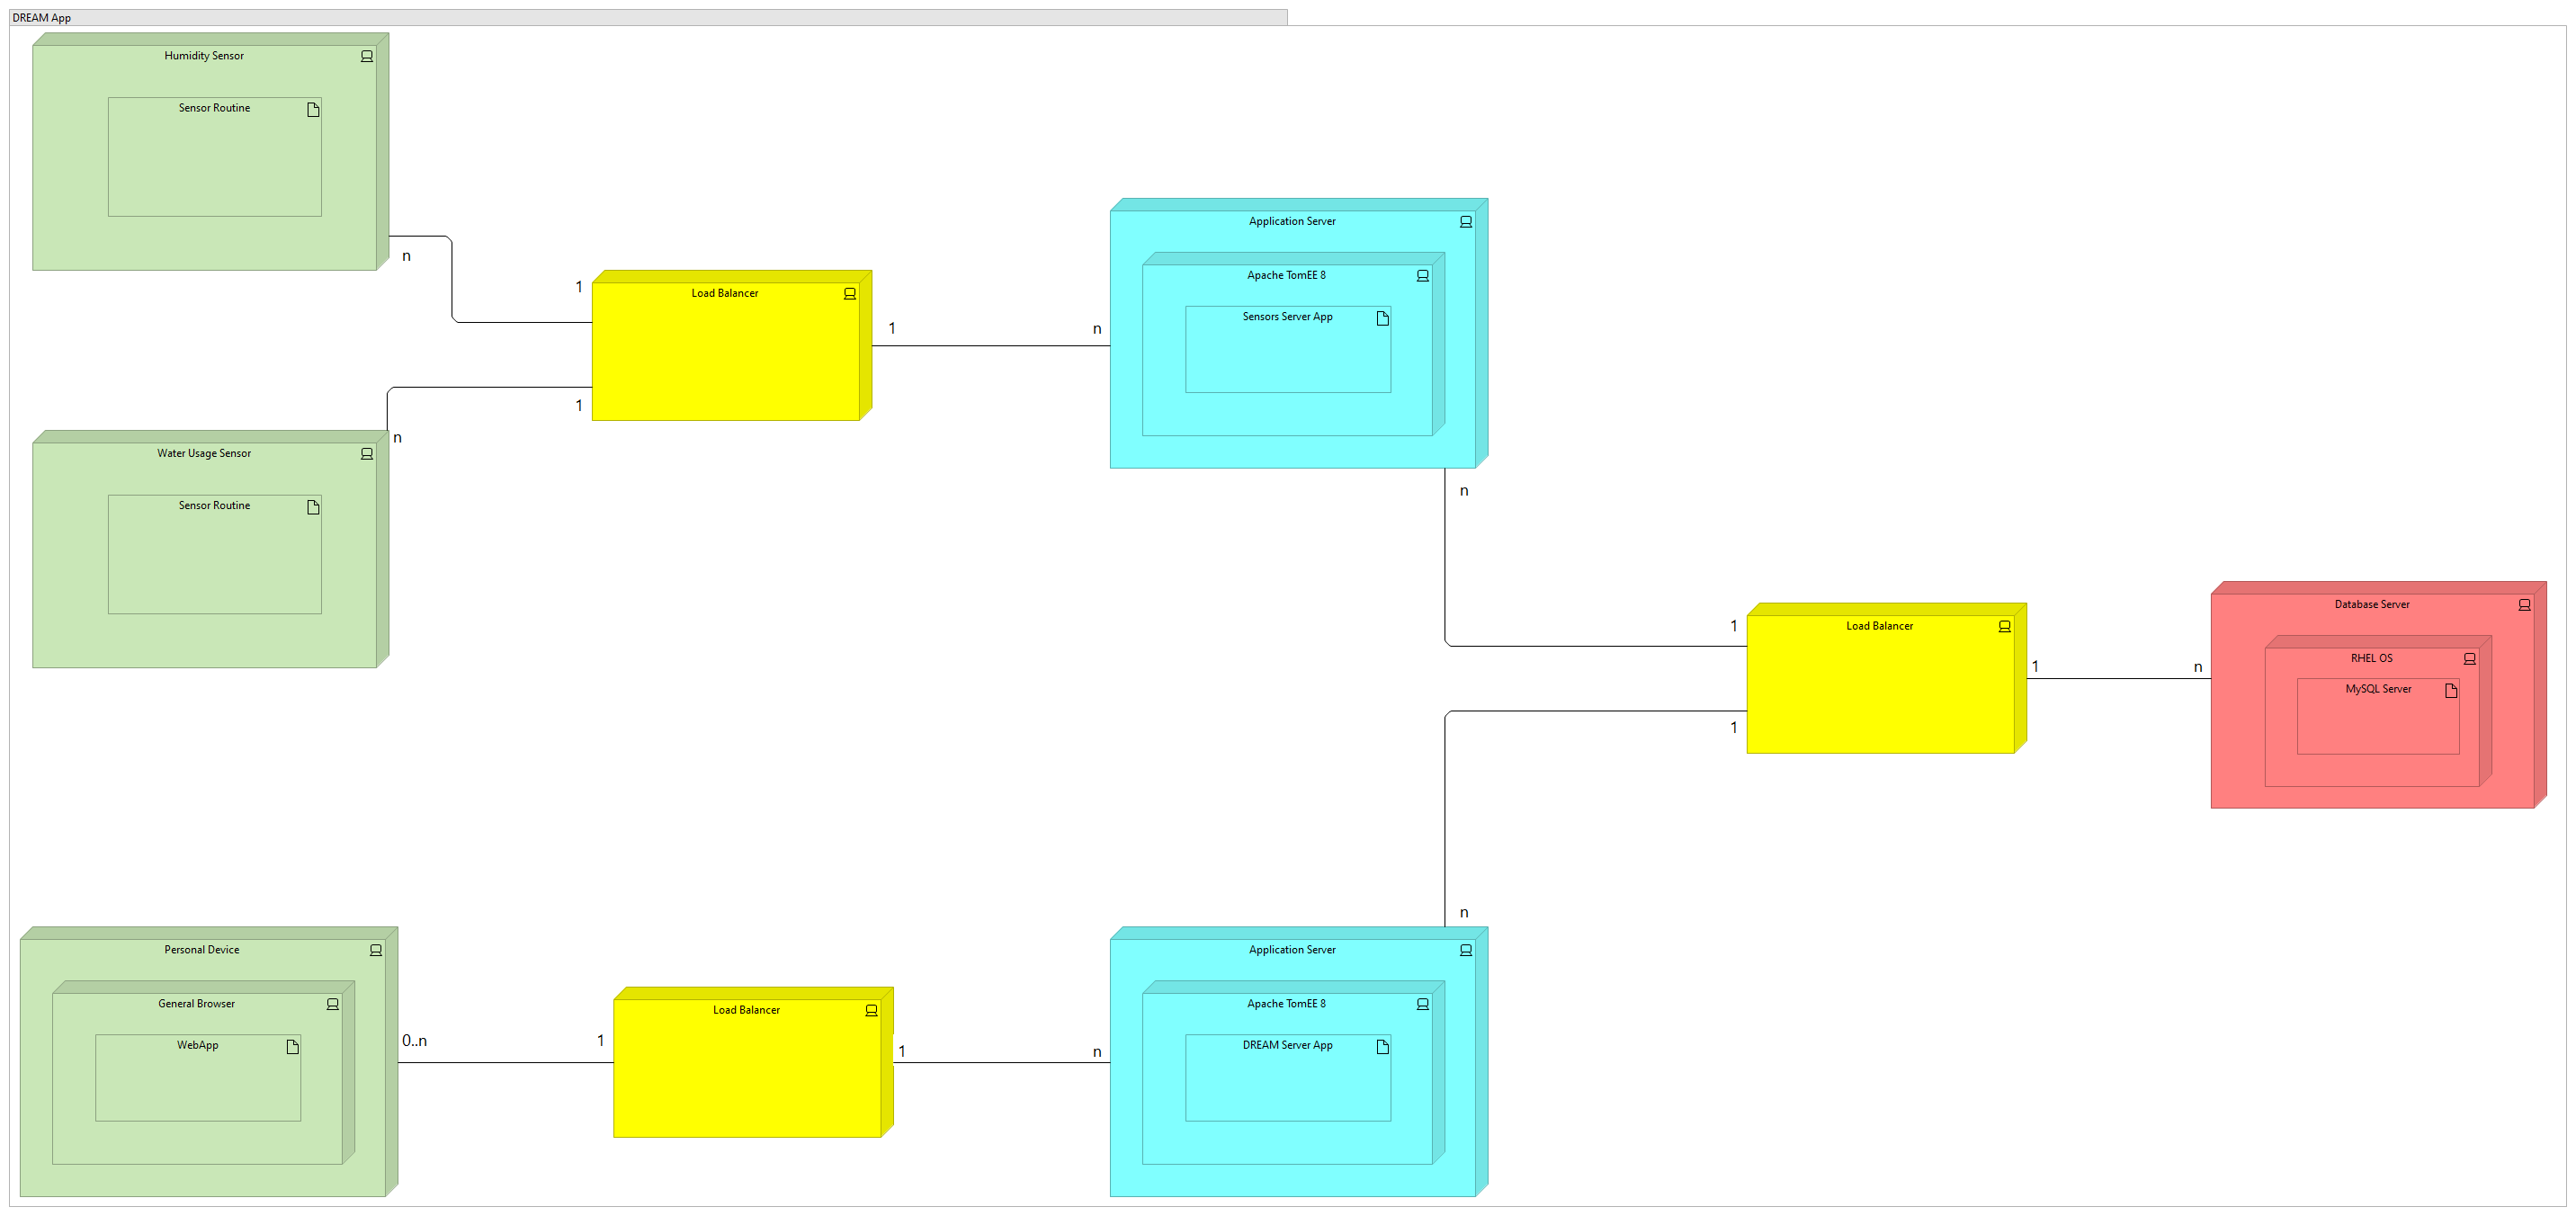
\includegraphics[width=\textwidth]{Images/DeploymentView.png}
    \caption{\textit{Deployment View of the System}.}
\end{figure}
\subsubsection{Presentation Tier}
The components of the presentation tier are presented below:
\begin{itemize}
    \item \textbf{Humidity Sensor and Water Usage Sensor: }These components only interact with the Sensors Server to send data acquired from their routine.
    \item \textbf{Personal Device: }DREAM’s system can be accessed from any device that utilizes any web browser. This will be the front-end layer, which consists of the user interface (this will be different for each role). The web-based approach has been chosen in order to guarantee access from any kind of device, with no restriction on the OS and without minimum requirements.
\end{itemize}
\subsubsection{Business Logic Tier}
The business logic tier contains the logic that drives the application’s core capabilities. The components are: 
\begin{itemize}
    \item \textbf{Sensor Server: }The role of this component is to receive the data routinely sent from the sensors and send them in an organized manner to the Third Tier, the database. The artifact for this component should be light, and it’s based on Apache TomEE 8.
    \item \textbf{DREAM Server: }This is the main logic component. This server has to manage each request from the First Tier, and it has to interact with the database to retrieve and update data. It also has the job to generate a different token for each role (i.e. Agronomists), which will then be used to show the correct user interface, and to guarantee access only to the allowed requests. The DREAM Server App is installed on a dedicated server with a running instance of Apache TomEE 8.
\end{itemize}

\subsubsection{Data Management Tier}
The data management tier comprises the database/data storage system and data access layer. Data is stored in a persistent way into a SQLServer database and accessed by the business logic tier via API calls.
\subsubsection{Load Balancer}
The role of the load balancers that divide the First and the Second Tier is to guarantee a correct load distribution between the multiple instances of the servers. Each server component can be duplicated in order to guarantee a more efficient managing of the requests. Both the Sensors Server and the DREAM Server could have as many instances as required, but in order to keep the system as light (and economic) as possible only two instances per server are required. This also provides an improved availability, since if only one of the two instances requires maintenance, the system can continue to work.\\
The load balancers that divide the Second and the Third Tier have a slightly different role. In fact, since many components require access to the database, either to retrieve data or to update it, three instances of the database are implemented, with one that act as a primary database and periodically sends “Sync Requests” to the replicas. This means that the load balancers will redirect every “write” operation to the primary database, while the “read” operations can be divided between the primary and the replicas.

\subsection{Run-time View}
\subsubsection{Login}
WebApp calls AuthManager, sending the credentials as parameters. AuthManager will then hash the password, and send the credentials to Model, which will create a query to verify the correctness of the data. If the inserted credentials are correct, both Model and WebApp will receive a token, which will then be used for every further interaction.
\begin{figure}[H]
    \centering
    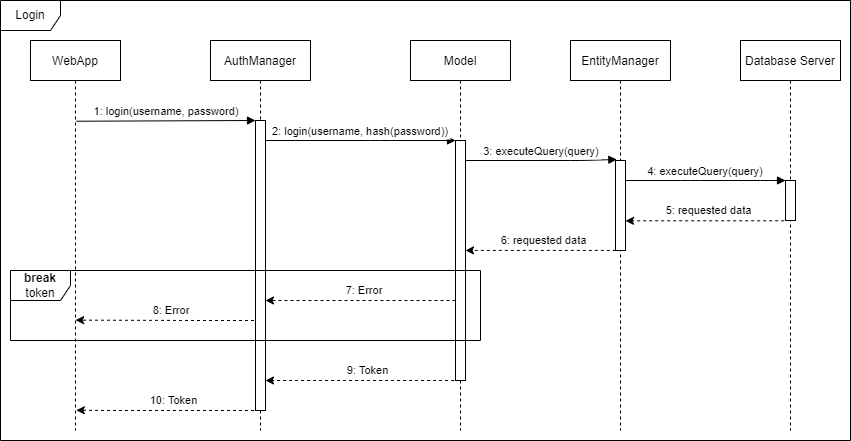
\includegraphics[width=\textwidth]{Images/Sequence Diagram/Login.png}
    \caption{\textit{LogIn} Sequence Diagram.}
\end{figure}
\newpage
\subsubsection{Sensor Interaction}
Sensors will routinely send the acquired data to the SensorController, which will send this information to the Model along with the type of sensor that sent the data. The model will then create the appropriate query to update the database, which will be executed by the EntityManager.
\begin{figure}[H]
    \centering
    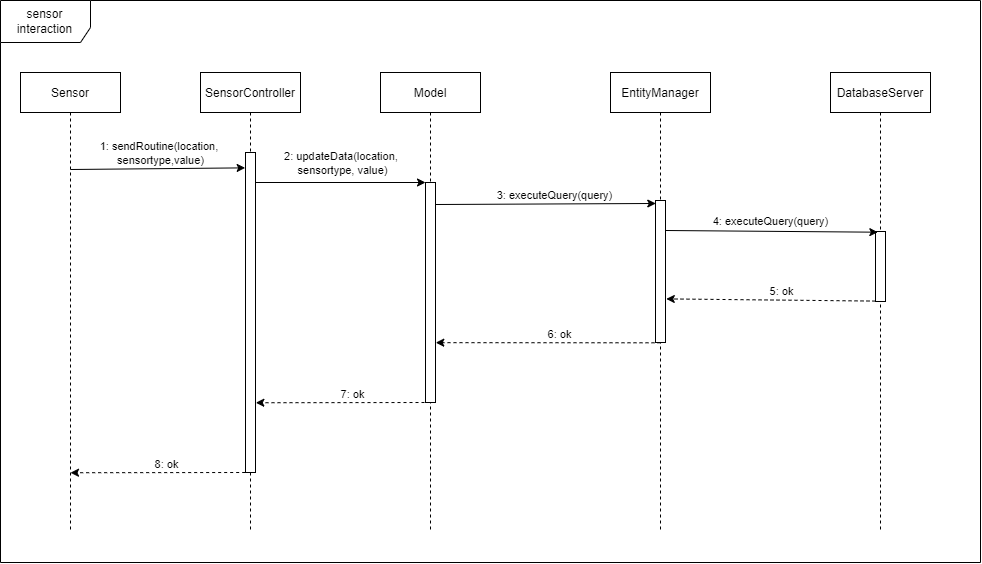
\includegraphics[width=\textwidth]{Images/Sequence Diagram/Sensor.png}
    \caption{\textit{Sensor} Sequence Diagram.}
\end{figure}
\newpage
\subsubsection{Report a Problem (Farmer)}
WebApp will send a request to FarmerManager, which will contain the title and the description of the problem, along with the token. FarmerManager sends the token to the Model, which verifies it and sends the result back to FarmerManager. This interaction happens every time a request is made by any user, and in order to improve readability it will not be reported in further diagrams. FarmerManager will then send to the Model the title and description of the problem, which will call ProblemManager in order to generate the query to insert it in the database.
\begin{figure}[H]
    \centering
    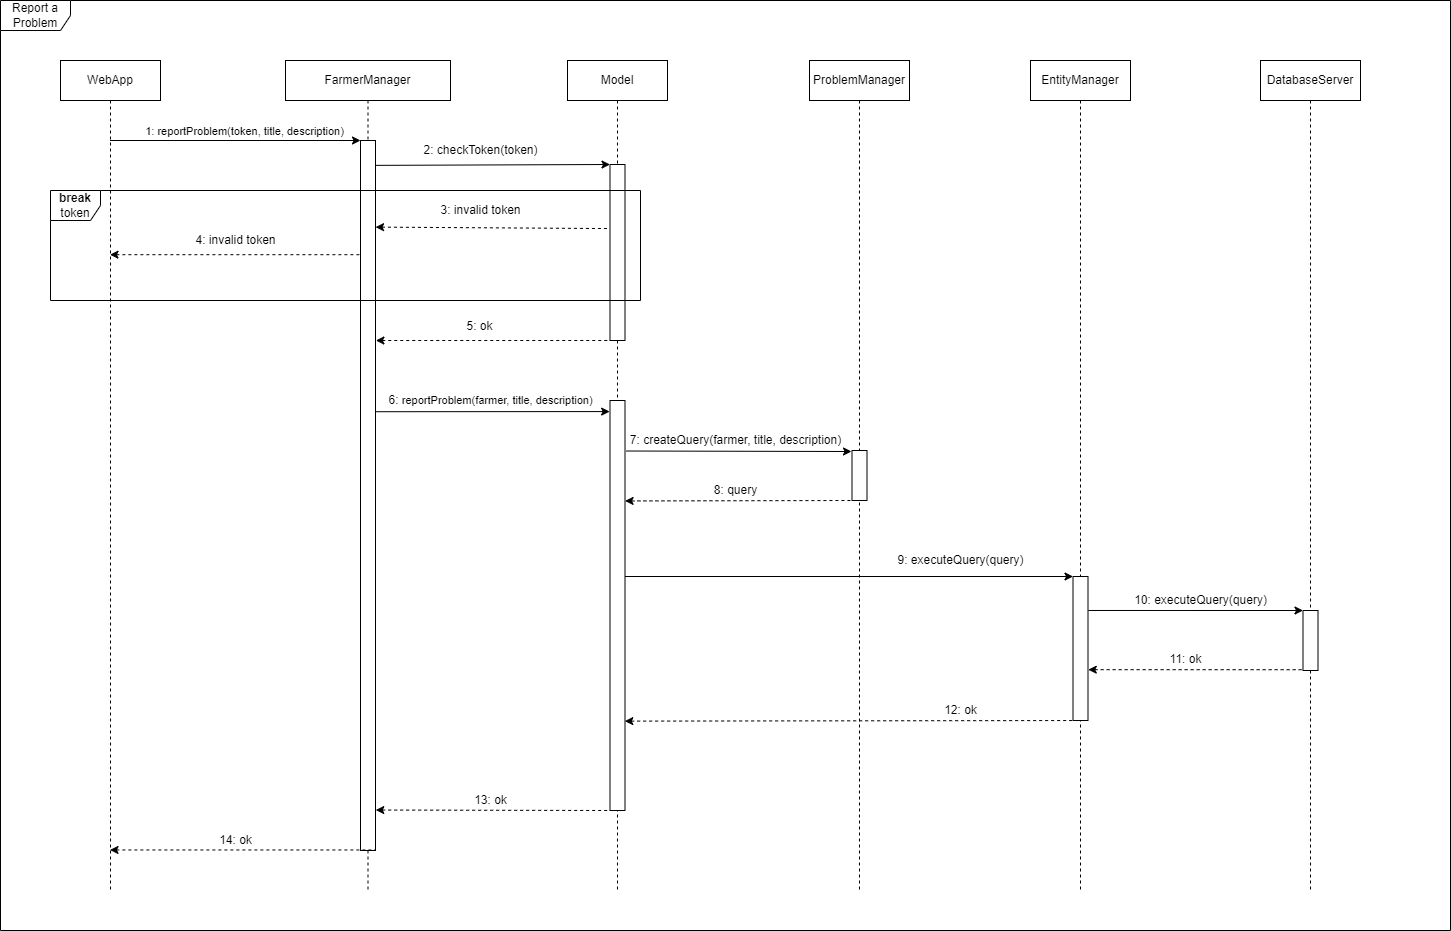
\includegraphics[width=\textwidth]{Images/Sequence Diagram/ReportProblem.png}
    \caption{\textit{Report a Problem(Farmer)} Sequence Diagram.}
\end{figure}
\newpage
\subsubsection{Report a problem (TPM/Agronomist)}
After the token is verified, Model calls ProblemManager in order to create the query to retrieve the list of problems reported in the selected zone. The user will select the problem to open, and, after the token gets verified again, ProblemManager creates the query to retrieve all the data concerning the problem.
\begin{figure}[H]
    \centering
    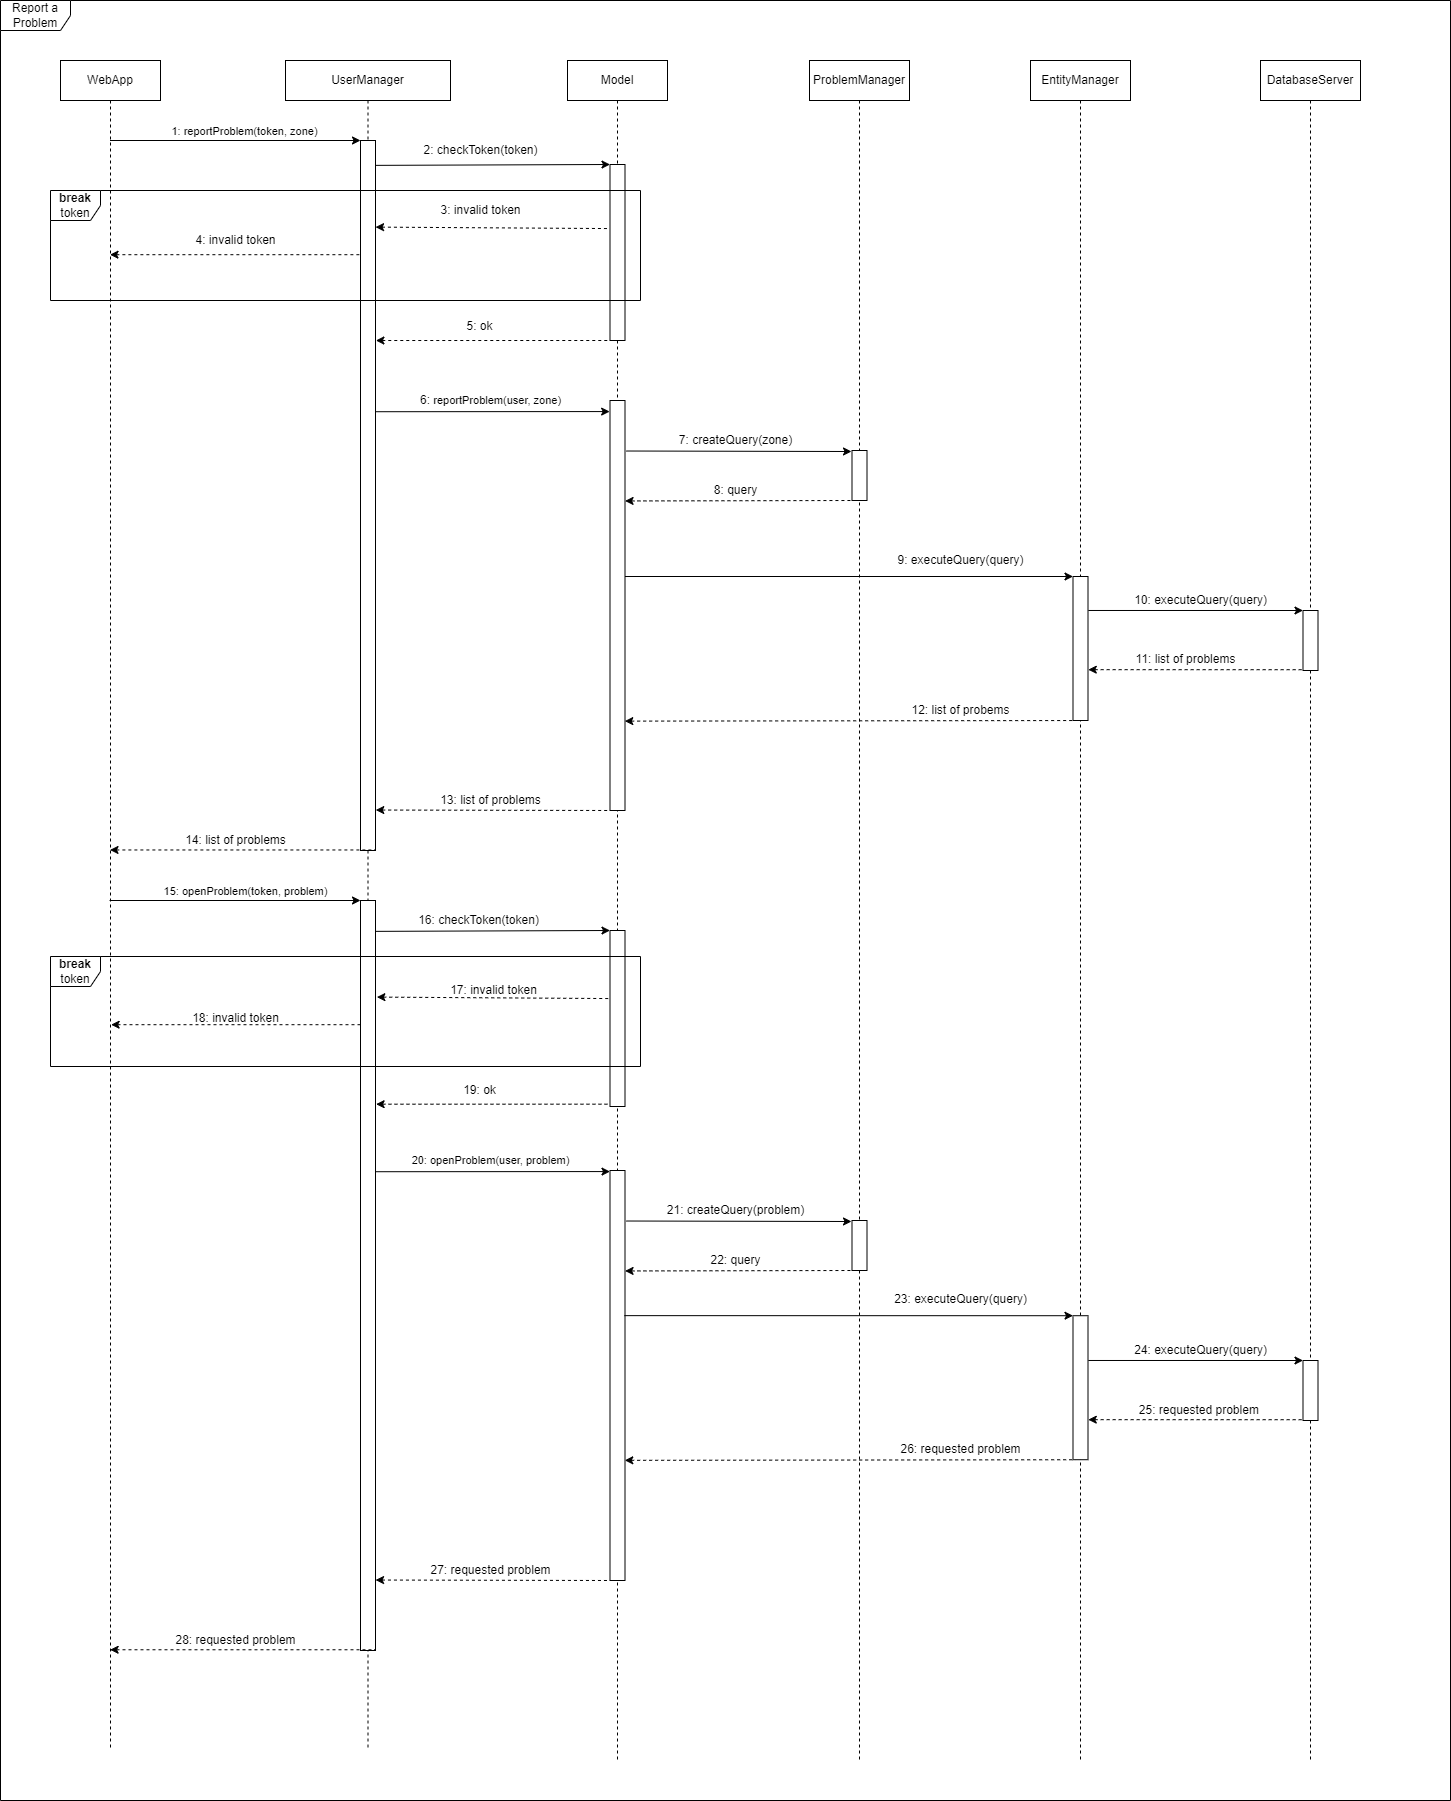
\includegraphics[width=\textwidth]{Images/Sequence Diagram/ReportProblemOthers.png}
    \caption{\textit{Report a Problem(Agronomist/TPM)} Sequence Diagram.}
\end{figure}
\subsubsection{WikiFarm}
After the token is verified, Model calls WikiFarm to create a query that selects the best performing farmers in the selected zone which have a cultivation with the selected type of production. The query will then retrieve the fertilizers and the seeds employed by these farmers.
\begin{figure}[H]
    \centering
    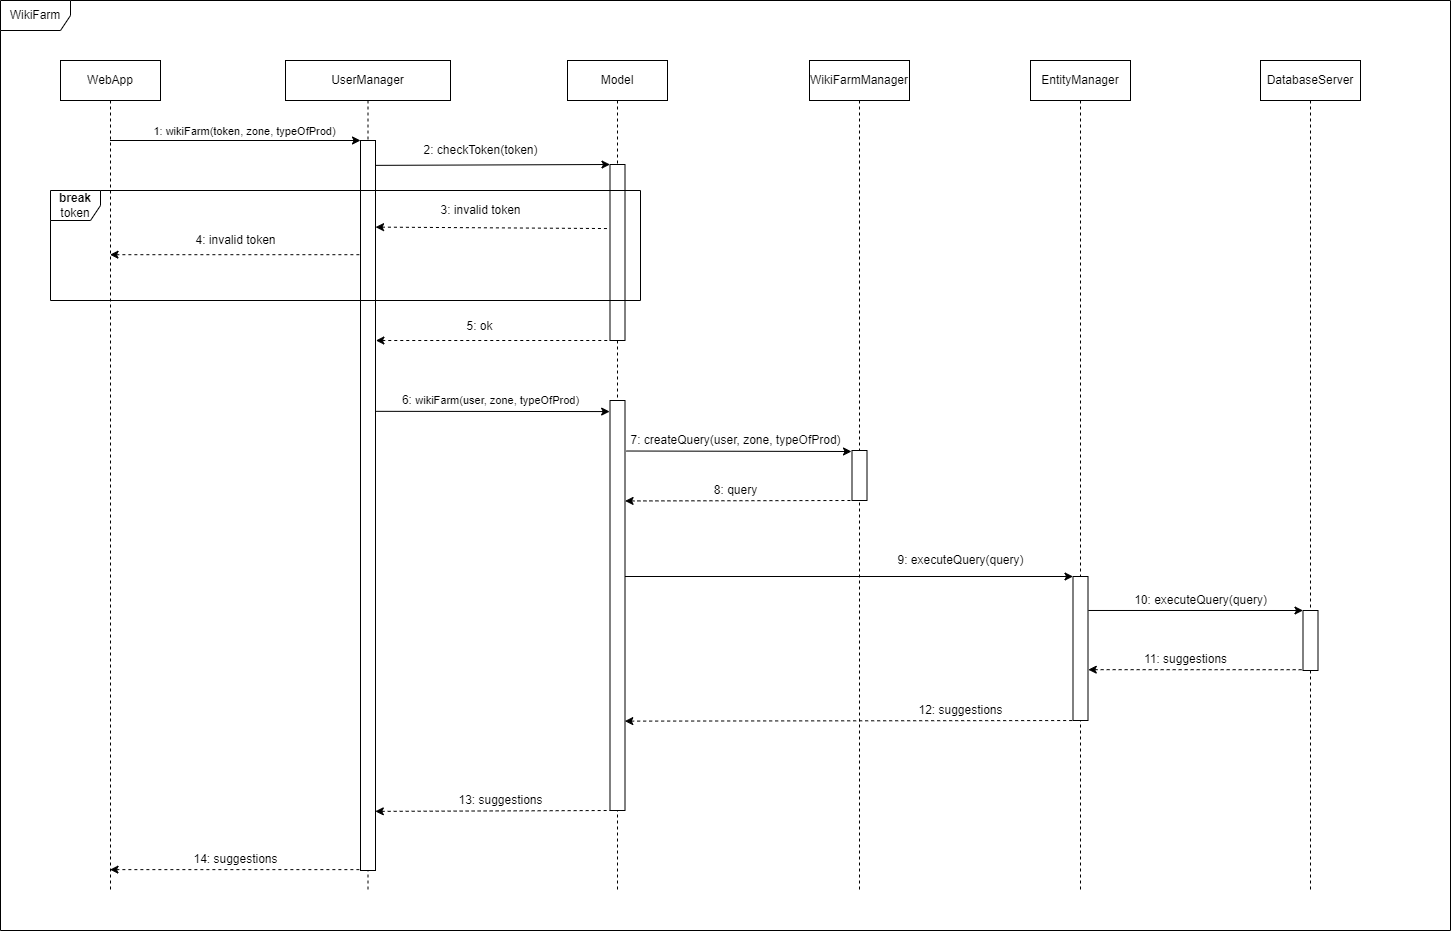
\includegraphics[width=\textwidth]{Images/Sequence Diagram/WikiFarm.png}
    \caption{\textit{WikiFarm} Sequence Diagram.}
\end{figure}
\newpage
\subsubsection{Weather}
After the token is verified, the Model calls WeatherManager, which interacts with WeatherService in order to retrieve the requested forecast.
\begin{figure}[H]
    \centering
    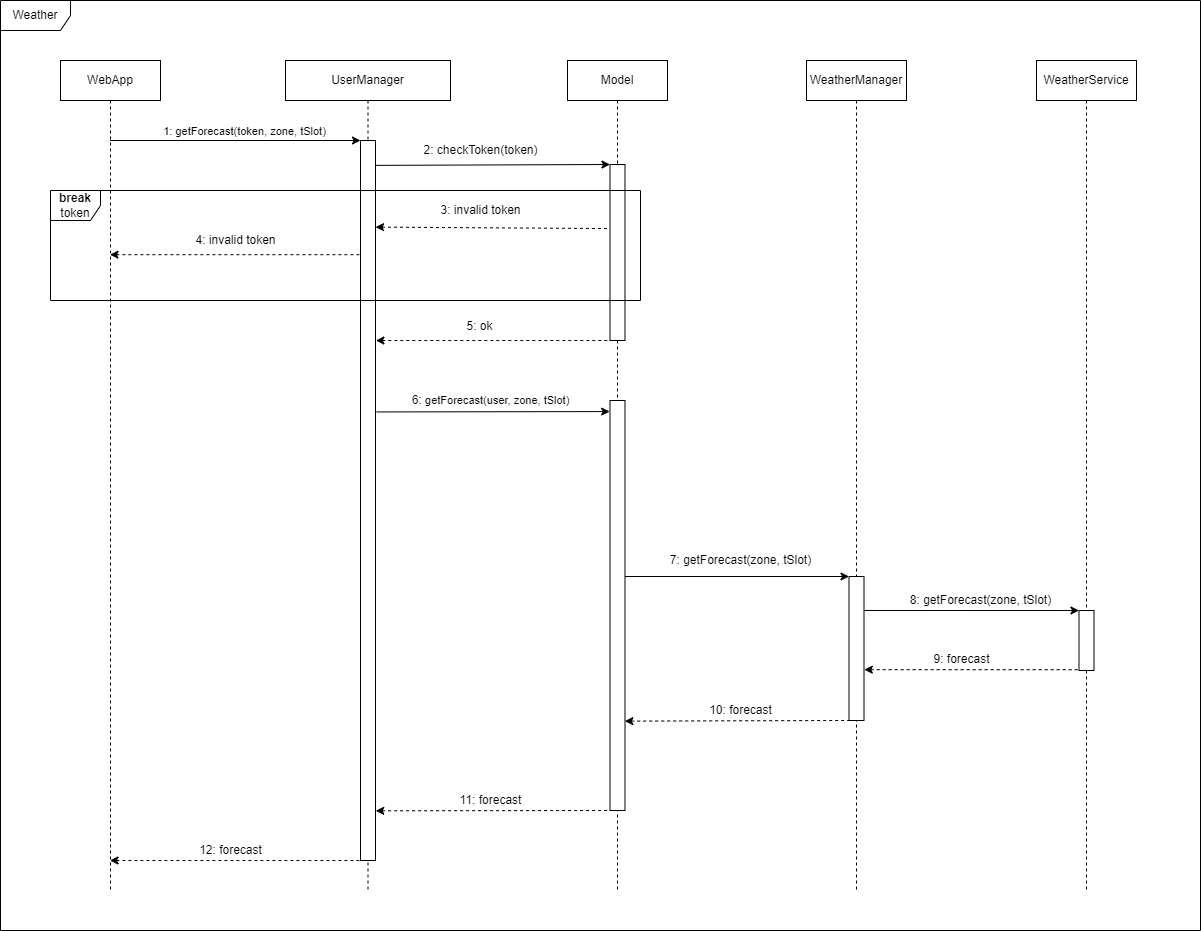
\includegraphics[width=\textwidth]{Images/Sequence Diagram/Weather.png}
    \caption{\textit{Weather} Sequence Diagram.}
\end{figure}
\newpage
\subsubsection{Report Production (Farmer)}
After the token is verified, the Model calls ProductionManager, which creates a query used to insert the reported production in the database.
\begin{figure}[H]
    \centering
    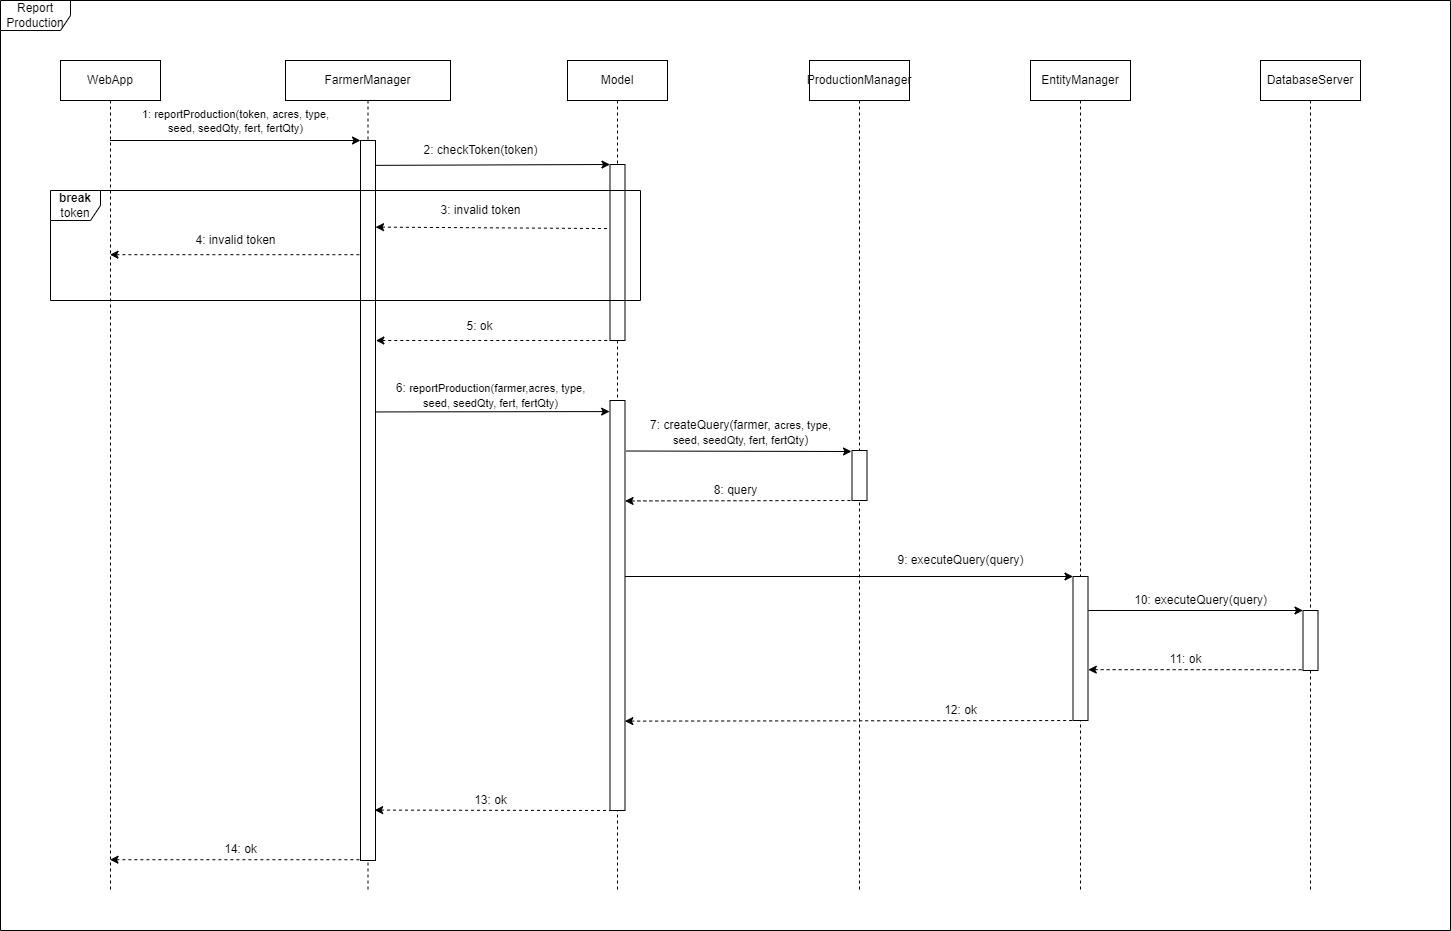
\includegraphics[width=\textwidth]{Images/Sequence Diagram/ReportProduction.png}
    \caption{\textit{Report Production (Farmer)} Sequence Diagram.}
\end{figure}
\newpage
\subsubsection{Report Production (Agronomist/TPM)}
After the token is verified, the Model calls ProductionManager, which takes the requested farmer as a parameter in order to generate a query to retrieve the reported productions. The token will then be verified again, and Model will call ProductionManager one more time, passing the selected report as a parameter. ProductionManager will then generate a query to retrieve all the data concerning the selected report.
\begin{figure}[H]
    \centering
    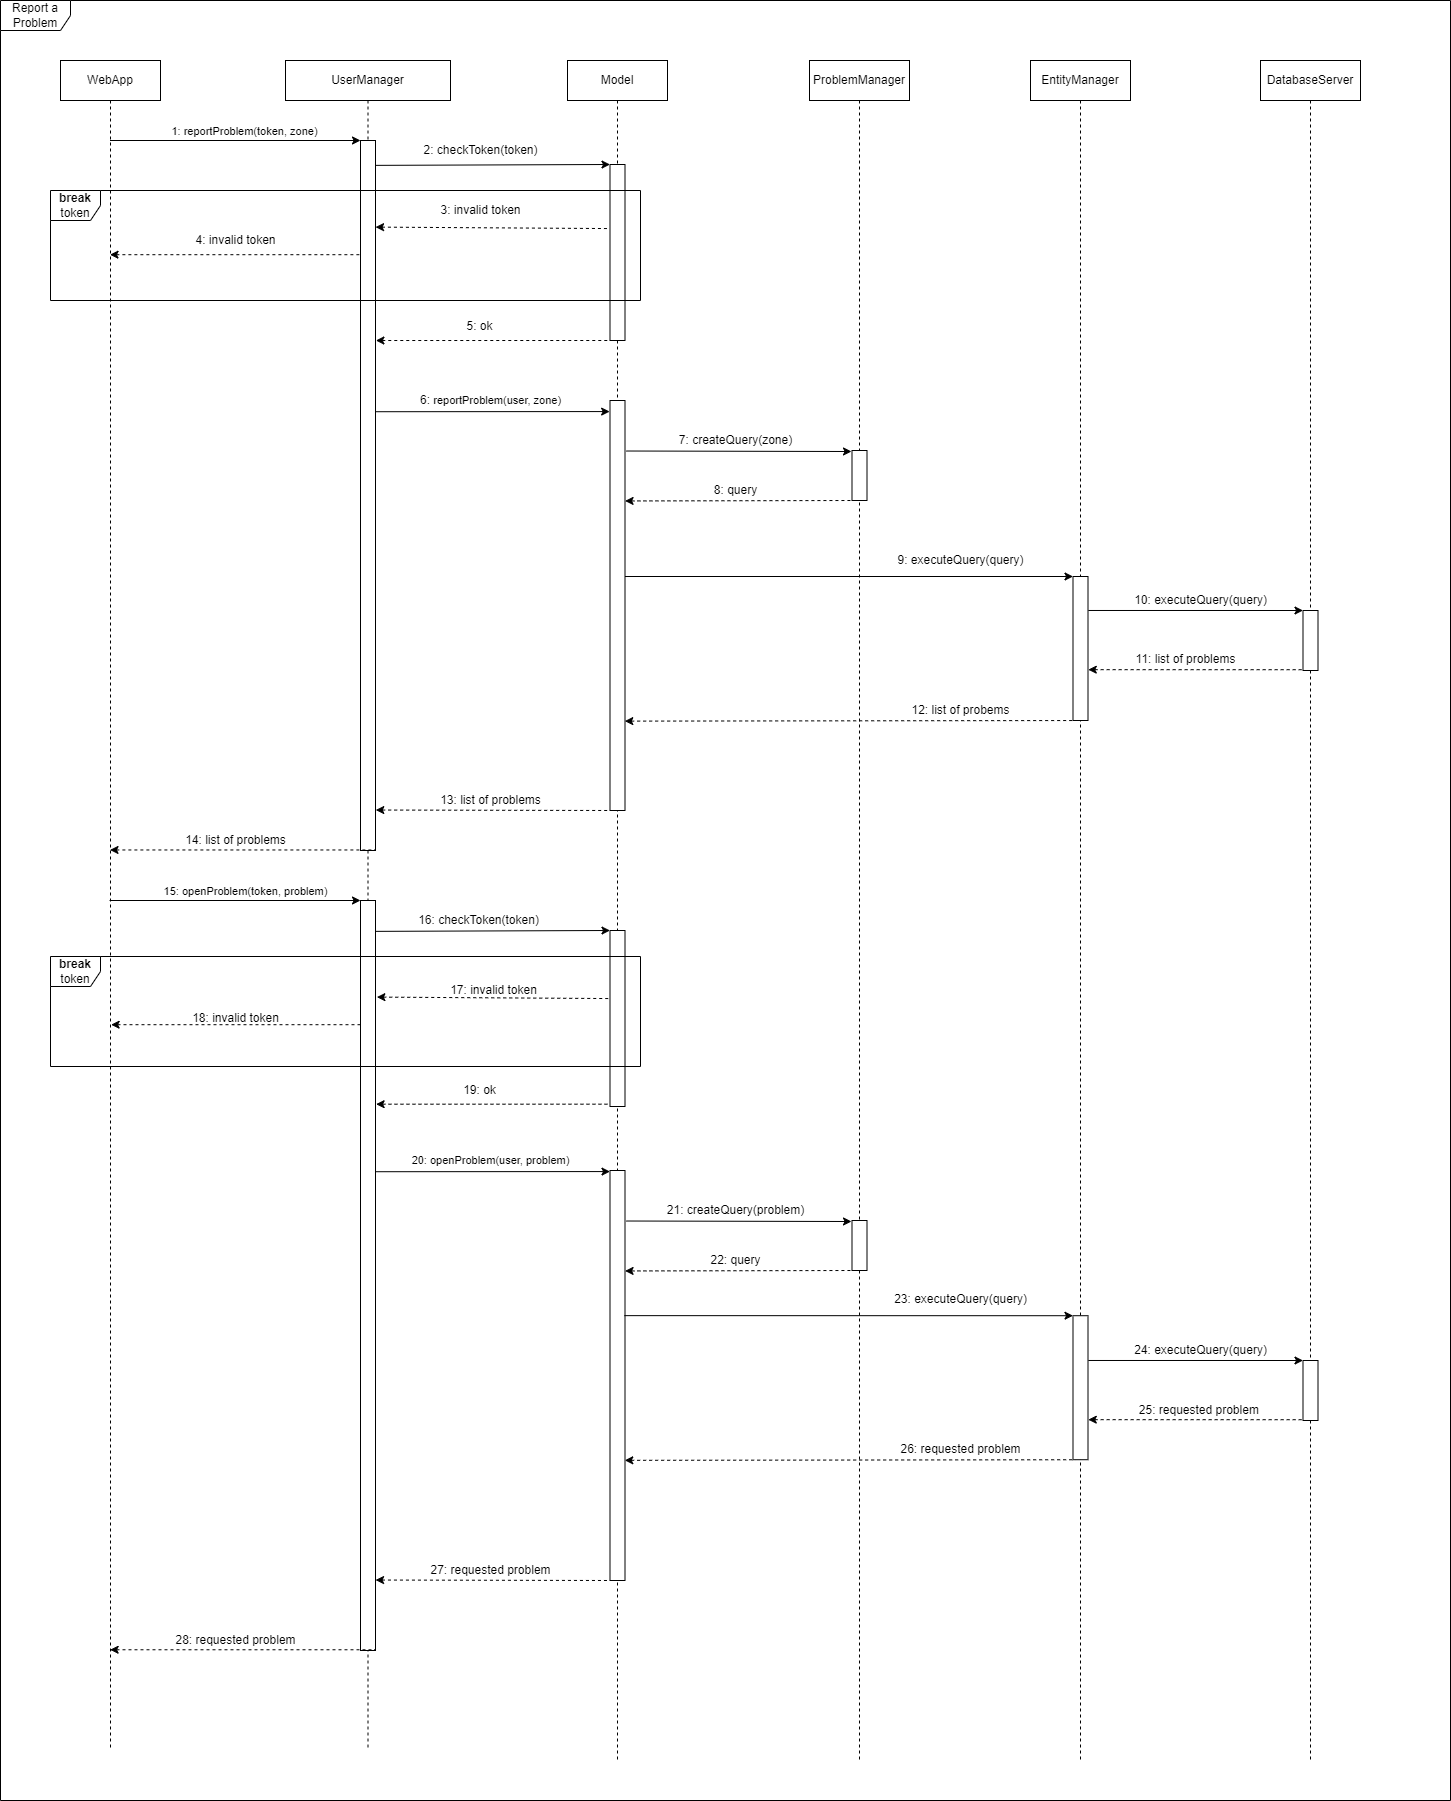
\includegraphics[width=\textwidth]{Images/Sequence Diagram/ReportProblemOthers.png}
    \caption{\textit{Visualize Production} Sequence Diagram.}
\end{figure}
\subsubsection{Help (Ask)}
After the token is verified, the Model calls HelpManager in order to generate a query to insert the request in the database.
\begin{figure}[H]
    \centering
    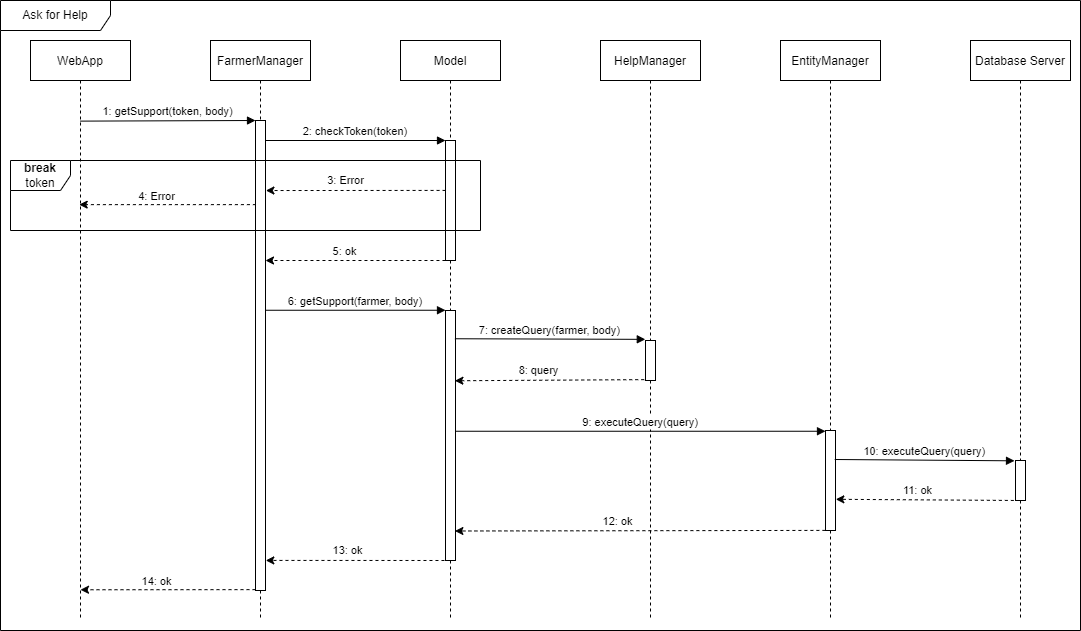
\includegraphics[width=\textwidth]{Images/Sequence Diagram/AskForHelp.png}
    \caption{\textit{Ask For Help} Sequence Diagram.}
\end{figure}
\subsubsection{Forum}
After the token is verified, the Model calls ForumManager in order to generate a query to insert the newly created discussion in the database.
\begin{figure}[H]
    \centering
    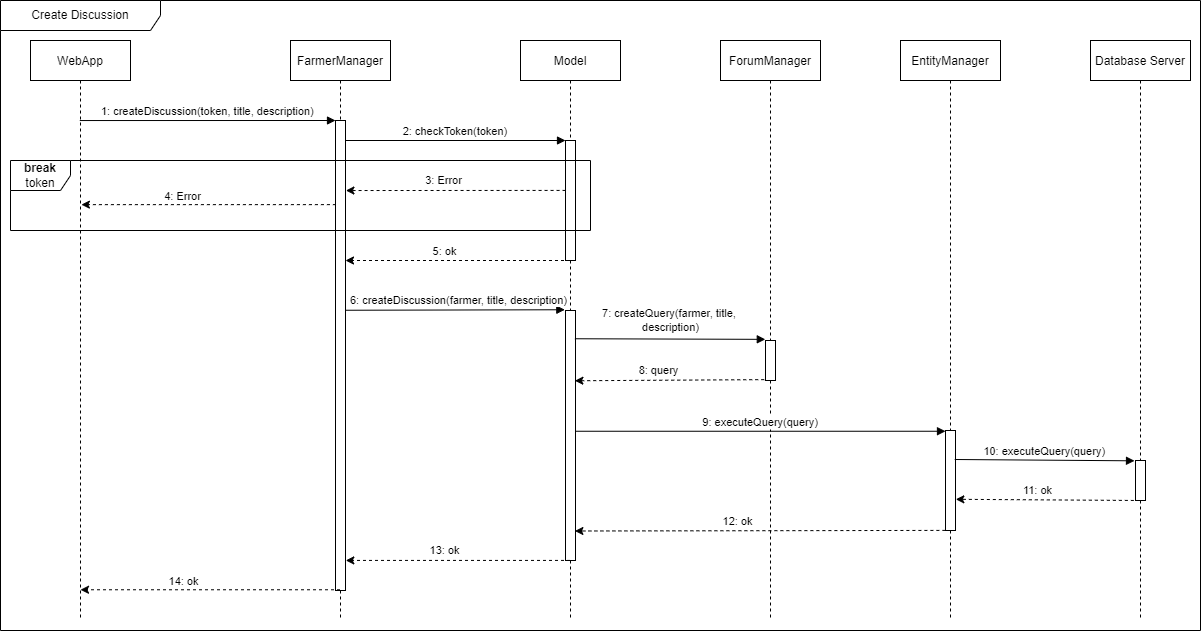
\includegraphics[width=\textwidth]{Images/Sequence Diagram/Forum.png}
    \caption{\textit{} Sequence Diagram.}
\end{figure}
\subsubsection{Agenda}
After the token is verified, the Model calls AgendaManager in order to create a query to insert the new event in the database.
\begin{figure}[H]
    \centering
    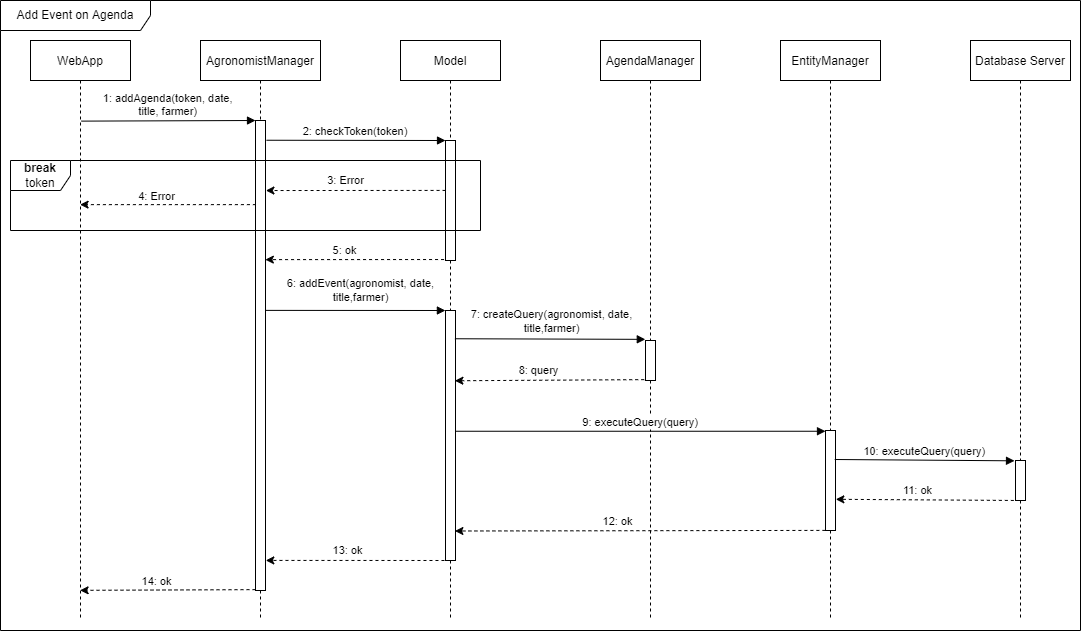
\includegraphics[width=\textwidth]{Images/Sequence Diagram/AgendaNewEvent.png}
    \caption{\textit{Creating a new Event} Sequence Diagram.}
\end{figure}
After the token is verified, the Model calls AgendaManager in order to create a query to retrieve all the planned events associated to the agronomists in the selected date
\begin{figure}[H]
    \centering
    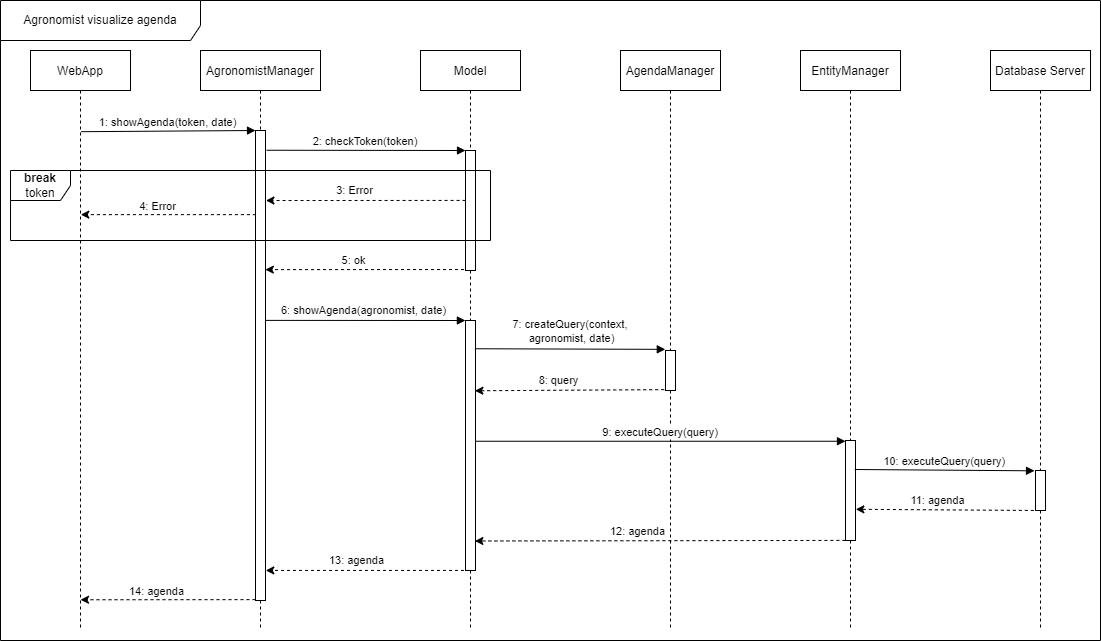
\includegraphics[width=\textwidth]{Images/Sequence Diagram/AgendaVisualize.png}
    \caption{\textit{Visualize Events} Sequence Diagram.}
\end{figure}
\subsubsection{Visualize Initiatives}
After the token is verified, the Model calls InitiativesManager in order to create a query to retrieve from the database all the reports associated to the requested farmer.
\begin{figure}[H]
    \centering
    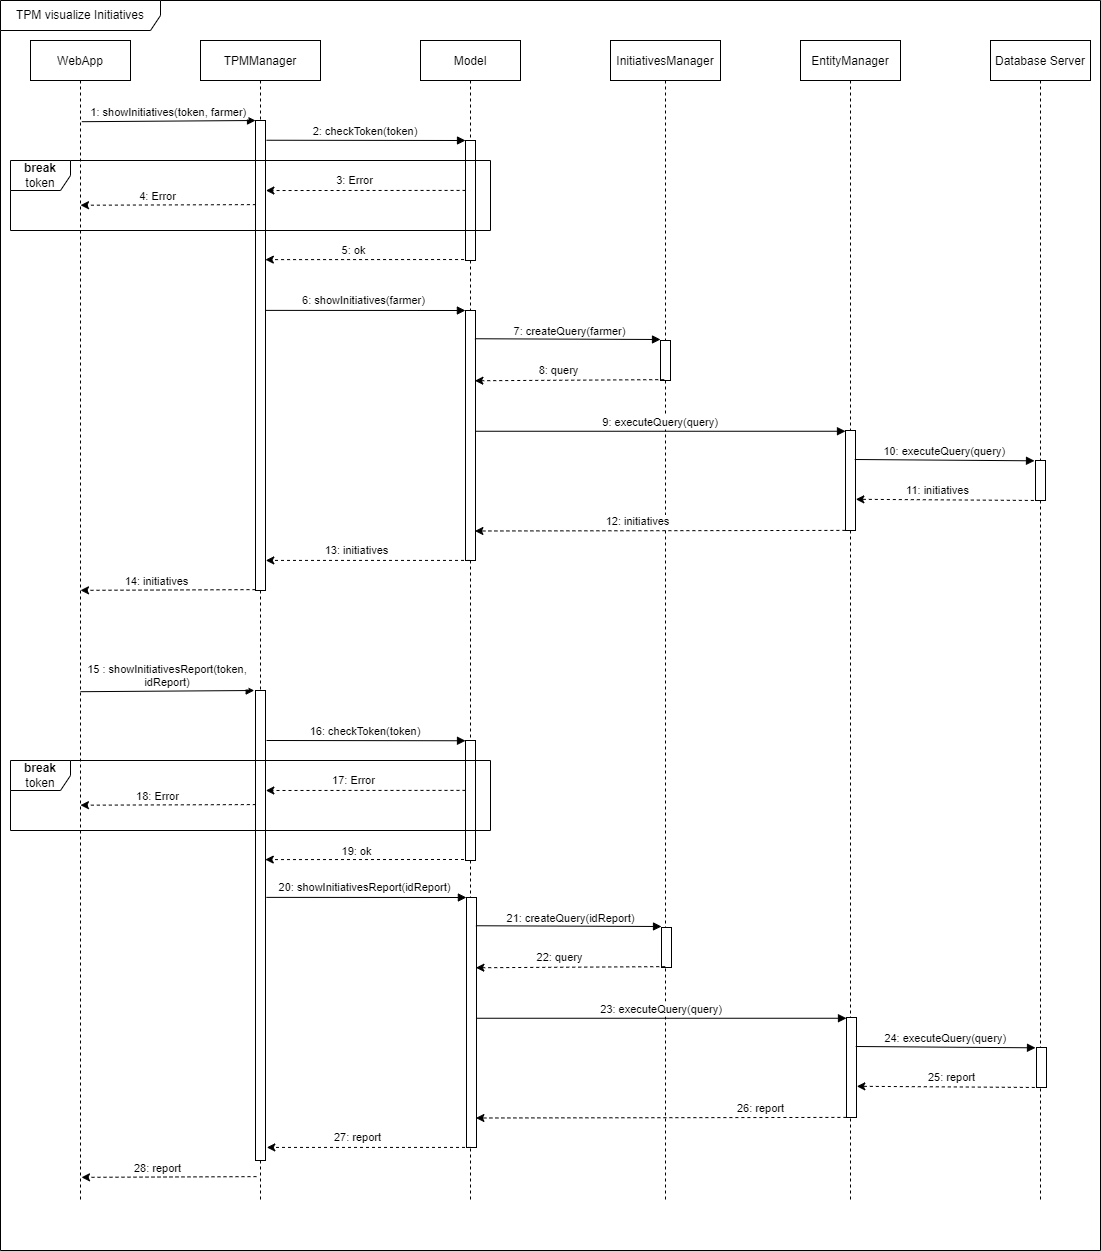
\includegraphics[width=\textwidth]{Images/Sequence Diagram/TPMVisualizeInitiatives.png}
    \caption{\textit{Visualize Initiatives} Sequence Diagram.}
\end{figure}
\newpage
\subsubsection{Ranking}
After the token is verified, the Model call RankingManager in order to create a query to retrieve the ranking of all the farmers associated to the selected zone. If no zone is selected, the query will request the global ranking.
\begin{figure}[H]
    \centering
    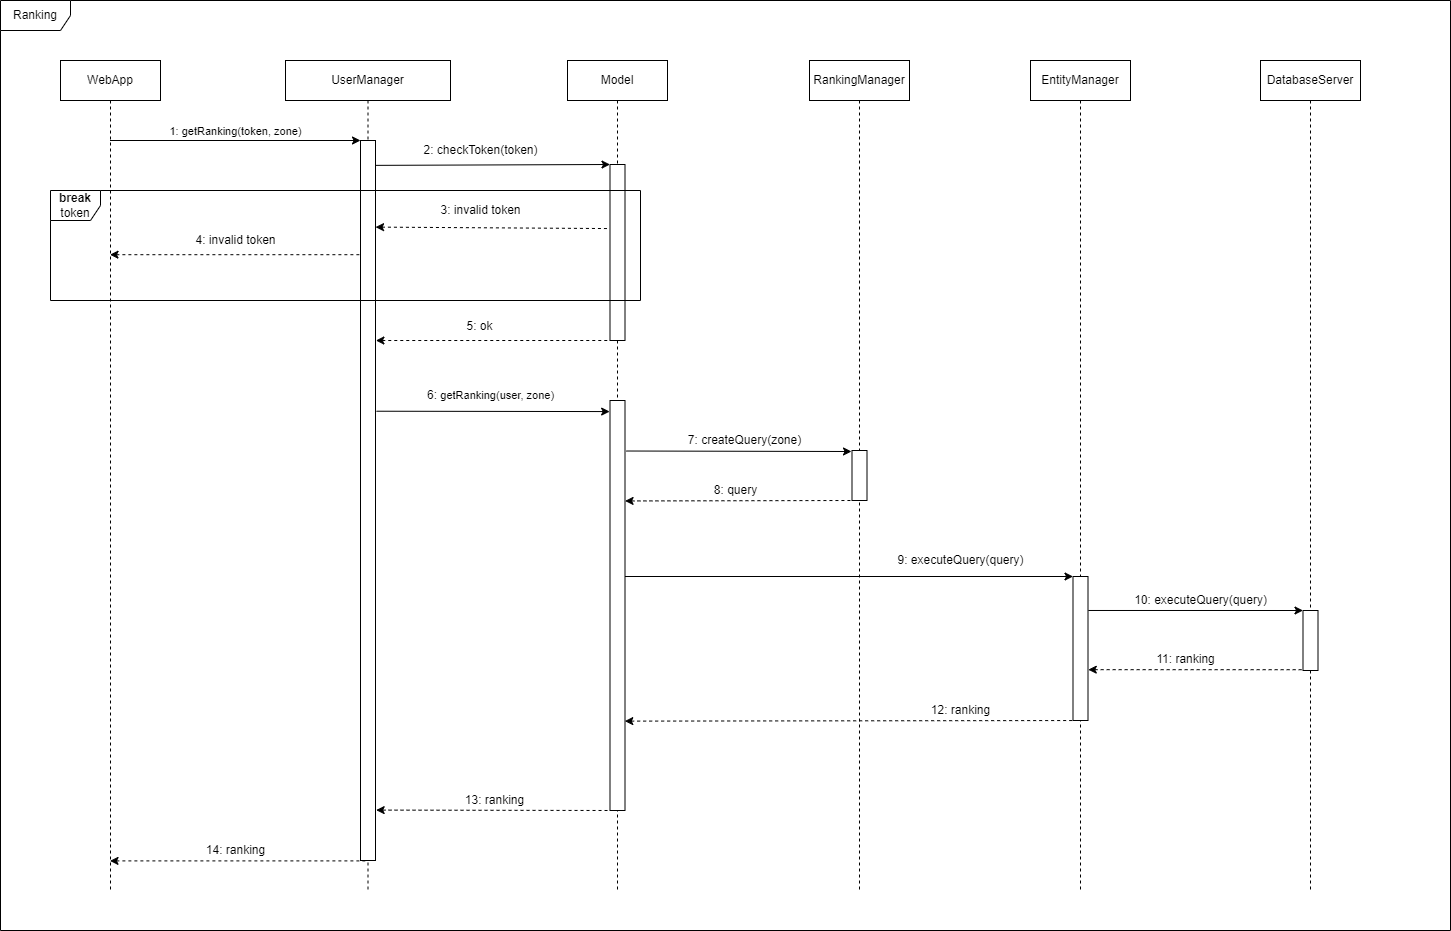
\includegraphics[width=\textwidth]{Images/Sequence Diagram/Ranking.png}
    \caption{\textit{Ranking} Sequence Diagram.}
\end{figure}
\newpage
\subsubsection{Chat}
This diagram represents WebApp1, which is a user that sends a message, and WebApp2, which is a user that visualize a message.
To send a message, the token has to be verified, then the Model will call ChatManager in order to generate a query that saves in the database the message, along with the receiver and the sender.
Instead, to visualize a message, the token has to be verified, then Model will call ChatManager in order to generate a query that retrieves all the messages associated to the user.
\begin{figure}[H]
    \centering
    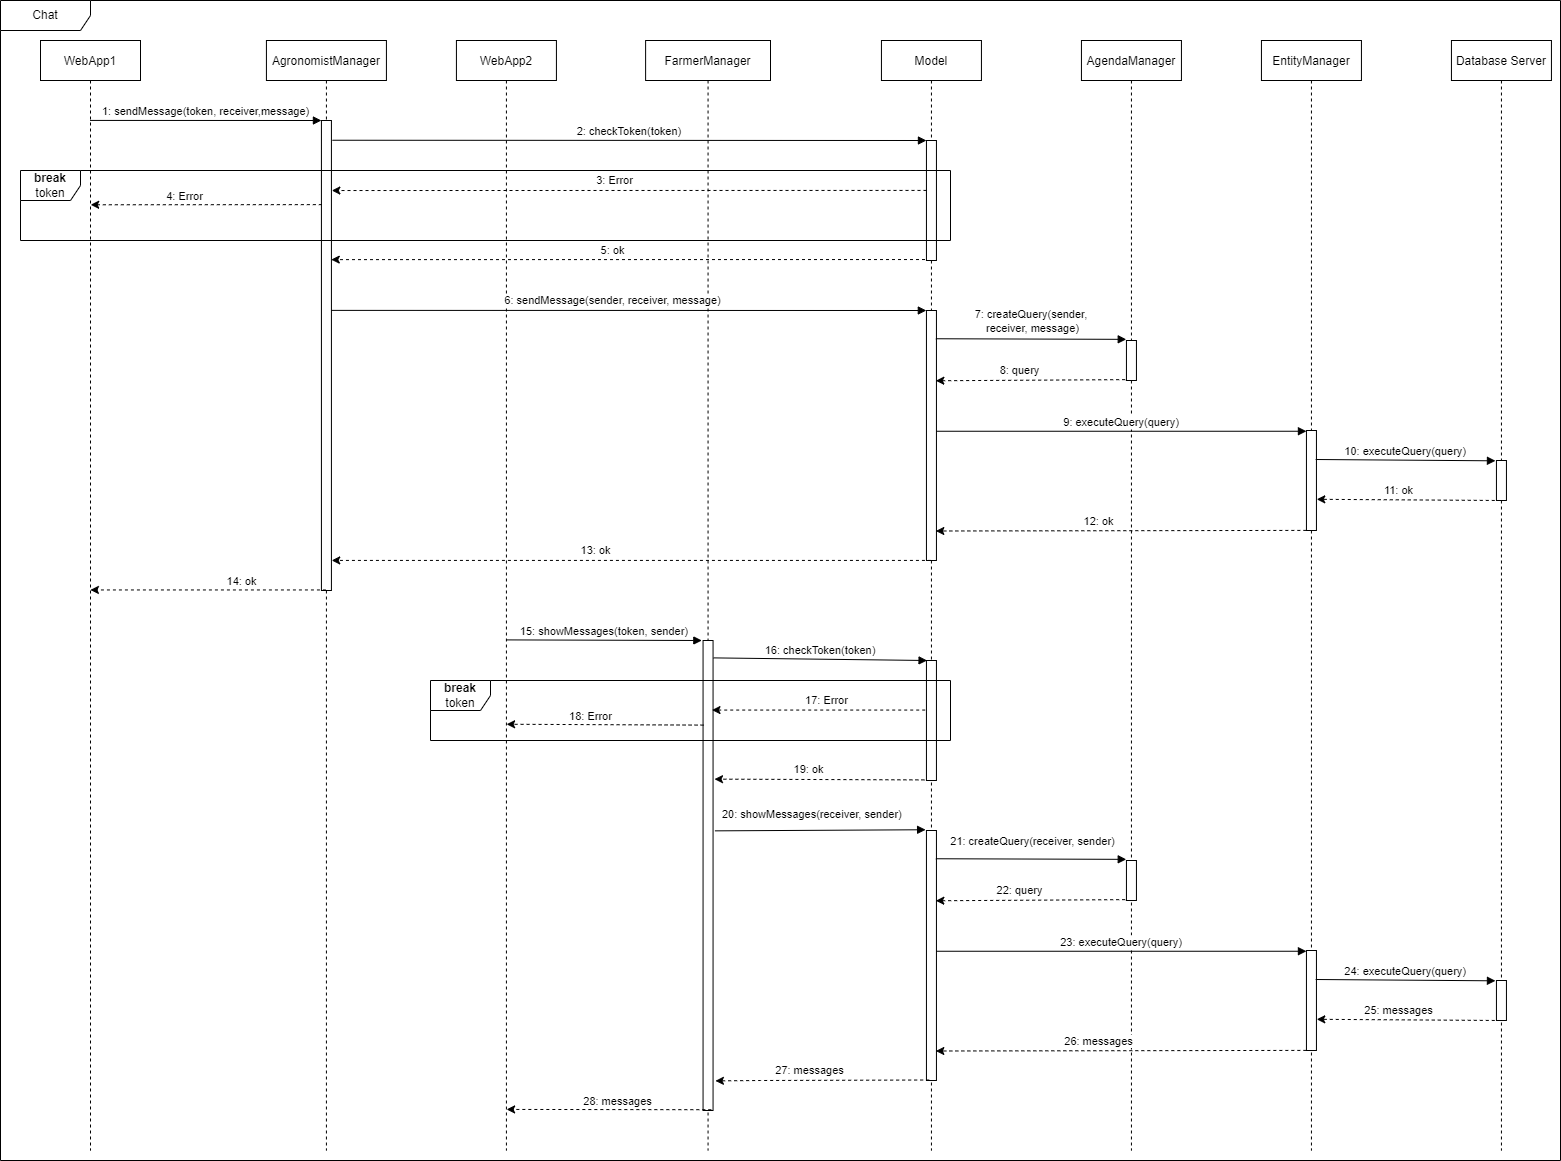
\includegraphics[width=\textwidth]{Images/Sequence Diagram/Chat.png}
    \caption{\textit{Chat} Sequence Diagram.}
\end{figure}
\newpage

\subsection{Component Interface}
This section lists all the methods that each component interface provides to the other components.
\subsubsection{DREAM Server}
\textbf{AuthManager}
\begin{itemize}
    \item login(username, password)
\end{itemize}
\textbf{FarmerManager}
\begin{itemize}
    \item getHomePage(token)
    \item getReportProblem(token)
    \item reportProblem(token, title, description)
    \item getHelpHomePage(token)
    \item getSupport (token)
    \item getSupport(token, body)
    \item openHelp(token)
    \item openHelp(token, idRequest)
    \item answerHelp(token, idRequest, answer)
    \item getForum(token)
    \item createDiscussion(token)
    \item createDiscussion(token, title, description)
    \item answerDiscussion(token, idDiscussion)
    \item answerDiscussion(token, idDiscussion, answer)
    \item getForecast(token)
    \item getForecast(token, zone, tSlot)
    \item wikiFarm(token)
    \item wikiFarm(token, zone, typeOfProd)
    \item reportProduction(token)
    \item reportProduction(token, acres, type, seed, seedQty, fert, fertQty)
    \item showChats(token)
    \item newChat(token)
    \item newChat(token, username)
    \item sendMessage(token, receiver, message)
    \item showMessages(token, sender)
\end{itemize}
\textbf{AgronomistManager}
\begin{itemize}
    \item getHomePage(token)
    \item getForecast(token)
    \item getForecast(token, zone, tSlot)
    \item showAgenda (token)
    \item showAgenda(token, date)
    \item addAgenda (token, date)
    \item addAgenda (token, date, title, farmers)
    \item showDetails(token, idVisit)
    \item editReport(token, idReport)
    \item editReport(token, idReport, report)
    \item setVisisted(token, idVisit)
    \item confirmDailyPlan(token, date)
    \item confirmDailyPlan(token, date)
    \item getProductionOthers(token, farmer)
    \item getProductionOthers(token, idReport)
    \item reportProblem(token)
    \item reportProblem(token, zone)
    \item openProblem(token, problem)
    \item wikiFarm(token)
    \item wikiFarm(token, zone, typeOfProd)
    \item showChats(token)
    \item newChat(token)
    \item newChat(token, username)
    \item sendMessage(token, receiver, message)
    \item showMessages(token, sender)
    \item getRanking(token, zone)
    \item openHelp(token)
    \item openHelp(token, idRequest)
    \item answerHelp(token, idRequest, answer)
\end{itemize}
\textbf{answerHelp(token, idRequest, answer)}
\begin{itemize}
    \item getHomePage(token)
    \item getRanking(token, zone)
    \item reportProblem(token)
    \item reportProblem(token, zone)
    \item openProblem(token, problem)
    \item showChats(token)
    \item newChat(token)
    \item newChat(token, username)
    \item sendMessage(token, receiver, message)
    \item showMessages(token, sender)
    \item getProductionOthers(token)
    \item getProductionOthers(token, farmer)
    \item getProductionOthers(token, idReport)
    \item showInitiatives(token)
    \item showInitiatives(token, farmer)
    \item showInitiativesReport(token, idReport)
\end{itemize}
\textbf{Model}
\begin{itemize}
    \item login(username, hashPassword)
    \item checkToken(token)
    \item reportProblem(farmer, title, description)
    \item reportProblem(user, zone)
    \item openProblem(user, problem)
    \item getSupport(farmer, body)
    \item openHelp()
    \item openHelp(idRequest)
    \item answerHelp(user, idRequest, answer)
    \item getForum()
    \item createDiscussion(farmer, title, description)
    \item answerDiscussion(idDiscussion)
    \item answerDiscussion(farmer, idDiscussion, answer)
    \item getForecast(user, zone, tSlot)
    \item wikiFarm(user, zone, typeOfProd)
    \item reportProduction(farmer, acres, type, seed, seedQty, fert, fertQty)
    \item getProductionOthers(user, farmer)
    \item getProductionOthers(user, idReport)
    \item showChats(farmer)
    \item sendMessage(sender, receiver, message)
    \item showMessages(receiver, sender)
    \item showAgenda(agronomist, date)
    \item addEvent(agronomist, date, title, farmers)
    \item showDetails(idVisit)
    \item editReport(idReport)
    \item editReport(idReport, report)
    \item setVisisted(idVisit)
    \item confirmDailyPlan(agronomist, date)
    \item getRanking(user, zone)
    \item showInitiatives(farmer)
    \item showInitiativesReport(idReport)
\end{itemize}
\textbf{RankingManager}
\begin{itemize}
    \item createQuery(zone)
\end{itemize}
\textbf{AgendaManager}
\begin{itemize}
    \item createQuery(context, agronomist, date)
    \item createQuery(agronomist, date, title, farmers)
    \item createQuery(context, idVisit)
    \item createQuery(idReport)
    \item createQuery(idReport, report)
\end{itemize}
\textbf{InitiativesManager}
\begin{itemize}
    \item createQuery(farmer)
    \item createQuery(idReport)
\end{itemize}
\textbf{ProductionManager}
\begin{itemize}
    \item createQuery(farmer, acres, type, seed, seedQty, fert, fertQty)
    \item createQuery(farmer)
    \item createQuery(idReport)
\end{itemize}
\textbf{WikiFarmManager}
\begin{itemize}
    \item createQuery(user, zone, typeOfProd)
\end{itemize}
\textbf{ProblemManager}
\begin{itemize}
    \item createQuery(farmer, title, description)
    \item createQuery(zone)
    \item createQuery(problem)
\end{itemize}
\textbf{HelpManager}
\begin{itemize}
    \item createQuery(farmer, body)
    \item createQuery()
    \item createQuery(idRequest)
    \item createQuery(user, idRequest, answer)
\end{itemize}
\textbf{ForumManager}
\begin{itemize}
    \item createQuery()
    \item createQuery(farmer, title, description)
    \item createQuery(idDiscussion)
    \item createQuery(farmer, idDiscussion, answer)
\end{itemize}
\textbf{ChatManager}
\begin{itemize}
    \item createQuery(farmer)
    \item createQuery(sender, receiver, message)
    \item createQuery(receiver, sender)
\end{itemize}
\textbf{EntityManager}
\begin{itemize}
    \item executeQuery(query)
\end{itemize}
\textbf{WeatherManager}
\begin{itemize}
    \item getForecast(zone, tSlot)
\end{itemize}

\subsubsection{Sensor Server}
\textbf{SensorController}
\begin{itemize}
    \item sendRoutine(location, sensortype, value)
\end{itemize}
\textbf{Model}
\begin{itemize}
    \item updateData(location, sensortype, value)
\end{itemize}
\textbf{EntityManager}
\begin{itemize}
    \item executeQuery(query)
\end{itemize}
\newpage

\subsection{Selected architectural styles and patterns}
Below are presented the decisions made during the design architecture.
\begin{itemize}
    \item \textbf{Three-tiers architecture: }As described in section 2.3, the system adopts this architecture to distinguish between client, server, and database.
    \item \textbf{Client-Server architecture: }This architecture has been used in conjunction with a thin client approach. A client makes a request for a service and receives a reply to that request; a server receives and processes a request and sends back the required response.
    \item \textbf{Model-View-Controller: }software design pattern that divides the program logic into three interconnected elements.
    \begin{itemize}
        \item Model: central component of the pattern. It is the application’s dynamic data structure, independent of the user interface. It directly manages the data, logic, and rules of the application.
        \item View: any visual representation of such as a chart, diagram, or table.
        \item Controller: responds to the user input and performs interactions on the data model objects. The controller receives the input, optionally validates it and then passes the input to the model.
    \end{itemize}
    \item \textbf{Adapter:} It’s a pattern used to match interfaces of different classes. The adapter is used as a middle layer between the UserManagers and the Model, as there is a unique interface that connects those components. E.g. FarmerManager will send a farmer object, while AgronomistManager will send an agronomist object, but they both use the same interface. 
    \item \textbf{Facade: }This pattern is used to create a component that offers an interface used to simplify and adapt the usage of another component. It’s used in the WeatherManager component to act as a connector with the external WeatherService.
    \item \textbf{Observer: }This is a way to notify a change to other classes. It’s used in the Chat function to implement the exchange of messages between two users. 
\end{itemize}
\newpage
%TODO: Non mi piace la grafica, più pulizia, e dobbiamo capire come metterla giù
\subsection{Other Design Decision}
\subsubsection{Database Structure}
All the data will be stored in a database implemented using SQLServer, since it is an open-source relational database management system.
The following diagram explains how the database is structured.
\begin{figure}[H]
    \centering
    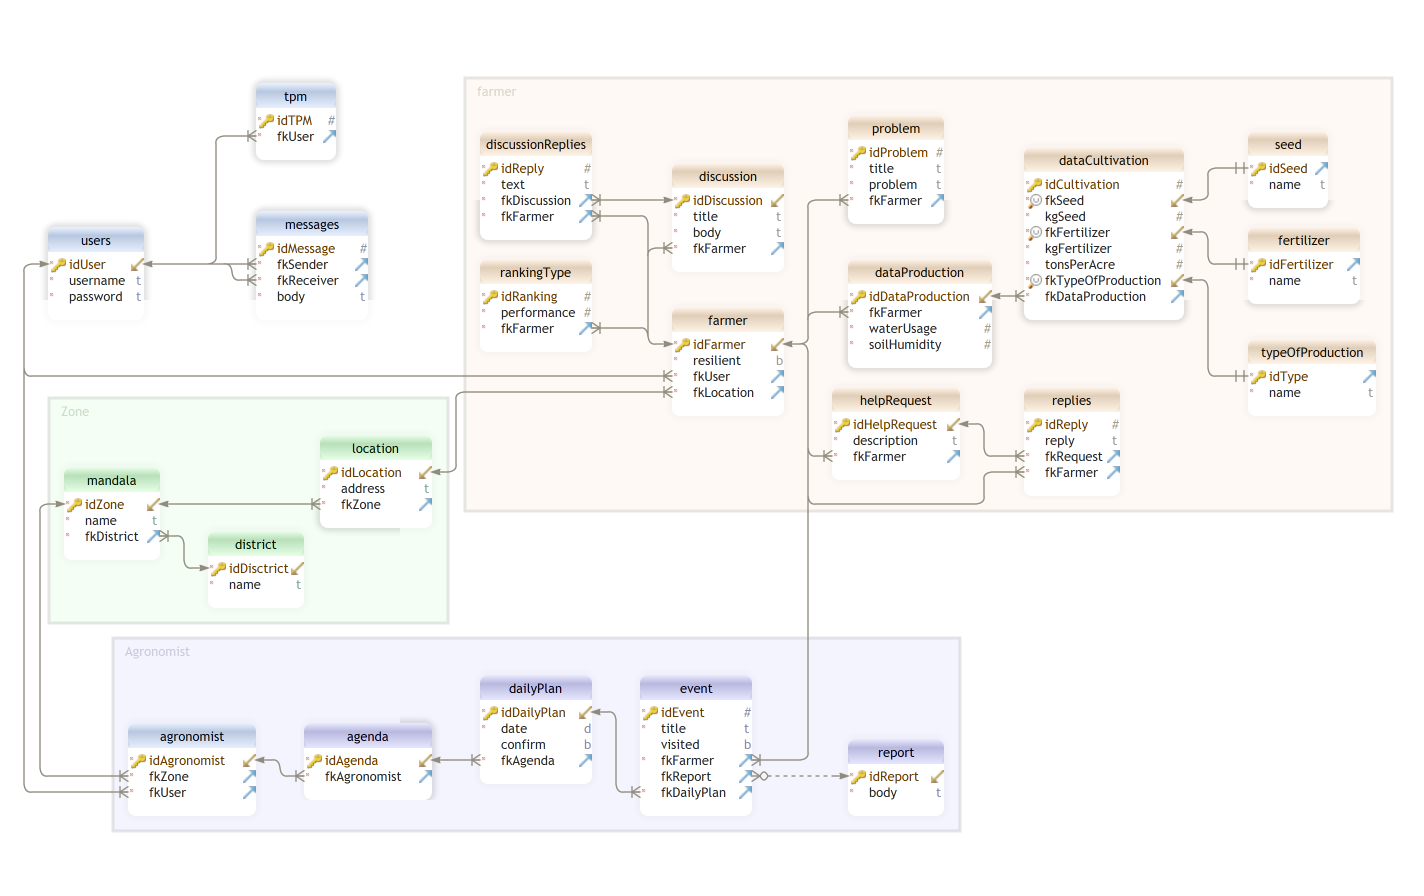
\includegraphics[width=\textwidth]{Images/DB_schema.png}
    \caption{\textit{Database Schema}.}
\end{figure}